\chapter{The Large Hadron Collider And the ATLAS Detector}
\label{chapter:ATLAS}

\epigraph{\textit{Please read carefully these precautions about the assembly.. When you finish assembling the product, please place it on a flat surface and make sure it is stable before use. Please also properly fix the anti-topple device, if included, in accordance with the assembly instructions. The product will keep longer by retightening the screws from time to time.}} {--IKEA, Assembly Instructions}

All data used in this thesis is taken from the ATLAS experiment~\cite{ATLAS:1999vwa} of the Large Hadron Collider(LHC)~\cite{Bruning:782076} in the European Organization of Particle Physics(CERN).

CERN is the largest research organization on particle physics in the world. (See Figure~\ref{fig:LHCOnBorder}for a schematic map) The laboratory was built in the 1950s as a joint European effort to advance particle physics. It includes a total of 23 member states to date. Many major physics discoveries were made at CERN. Most notably, the discovery of the W, the Z boson~\cite{hioki1982does}, and the first man-made antihydrogen atom~\cite{hioki1982does}. In 2012, a boson of mass 125
$\textit{GeV}/\textit{c}^{2}$ was discovered, it is believed that it matches the
profile of the long sought after Higgs Boson particle~\cite{chatrchyan2012observation}, which gives an explanation to the origin of mass of matter in the universe. The site with 2660 on-site personnels and 12,400 users from over 70 countries also produced many technological derivatives outside of scientific discoveries. In particular, the World Wide Web was first built at CERN~\cite{berners1994world}.

This chapter presents the hardware and software apparatus in the LHC at CERN used to collect and produce the datasets for the later analyses.
The working and the layout of the LHC, the machine used to accelerate protons and monitor its collisions is presented in Section~\ref{LHC}; the ATLAS detector, the apparatus used to collect proton-proton collision data is described in Section~\ref{ATLAS}. Lastly, the triggering chain: the hardware and software collecting strategy is presented in Section~\ref{trigger}.

\begin{figure}[!htb]
    \begin{center}
        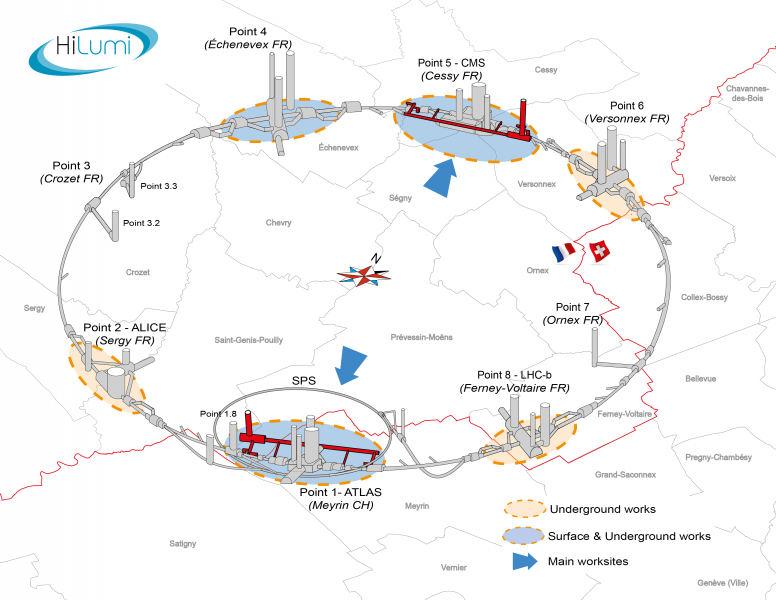
\includegraphics[width=0.75\textwidth]{figures/chapter_ATLAS/LHCOnBorder}
        \caption{
            This figure shows where the CERN is located geographically, across the border between France and Switzerland~\cite{Bruning:782076}.
        }
        \label{fig:LHCOnBorder}
    \end{center}
\end{figure}

\section{The Large Hadron Collider}
\label{LHC}

The LHC is located on the France-Switzerland border. Its main ring is a 27 kilometers tunnel that is 175 meters underground. It is mainly used to collide protons. Lead-lead collisions and proton-lead collisions are also done for a few weeks in each data-taking year. 

The collider was a planned successor to the Large Electron-Positron (LEP)(209 GeV collision) and the Tevatron collider (up to 1.96TeV) in Fermilab. Since the last two experiments, the community converged on a consensus of an O(10)TeV scale proton collider with the main physics goal to probe electro-weak scale Higgs boson, beyond-the-Standard-Model physics, and further Standard Model measurement studies. The LHC was born.

The LHC reuses the same tunnel as the LEP experiment, with some major modifications were done to the tunnel for the upgrade: to achieve higher center-of-mass energy and to collide proton-proton instead of electron-positron, the angular velocity of the particle colliding would need to be raised. The existing magnet from the LEP experiment was therefore replaced to make way for more powerful cryogenic-based super-conducting magnets to bend higher speed particles. In addition, as the LHC uses a proton-proton beam rather than an electron position in the LEP, an extra beam pipe was required. This is due to the fact that the proton beams collisions could not share the same beam pipe as the position-electron beams in the LEP. The radio frequency system is also modified in the upgrade to the LHC to allow for acceleration of the two separate beams in the LHC.

After the upgrade, the main ring of the LHC allows for particle collision to happen in four main intersection points. These four points are directly inside the four major experiments of ATLAS~\cite{ATLAS:1999vwa}, CMS~\cite{CMS:2006myw}, LHCb~\cite{lhcb2001technical} and ALICE~\cite{Cortese:519145}: 

ATLAS and CMS are general-purpose detectors, data collected from these experiments are used for studies including Standard Model measurement, Higgs property measurement as well as exotic and new physics searches. The similar but slightly different detector structure between the two experiment allow for crosschecks and validation of physics results. ALICE is optimized to study strong physics in the quark-gluon plasma generated from lead-lead collisions. LHCb is a forward detector that specializes in b(bottom quark)-physics measurement. Studies on the bottom quark done in LHCb measures CP violation parameter and could help better understand matter-antimatter asymmetry of the universe. 

In addition to the four major experiments, the LHC currently hosts four more experiments. LHCf looks for forward particles that originate from cosmic radiation~\cite{Adriani:926196}. FASER is an experiment in search of long-lived exotic particles with a lifetime beyond the ATLAS detector~\cite{Ariga:2651328}. MoEDAL, which sits in the cavern of LHCb, looks for the magnetic monopole or highly ionizing stable massive particles (SMP)~\cite{Pinfold:1181486}. TOTEM shares the CMS interaction point; it measures the total
cross-section, diffraction process and elastic scattering processes of particles in the proton collisions~\cite{TOTEM:2004hps}. 

The LHC is designed to operate at a maximum center-of-mass energy of 14 TeV. Protons that get collided at the different interaction points go through many stages before collisions. 

In the following sections, some technical terms related to LHC operation will be discussed. Different parts of the LHC from proton production, proton acceleration to proton collision in the center of the ATLAS detector is also covered.

\begin{figure}[!htb]
    \begin{center}
        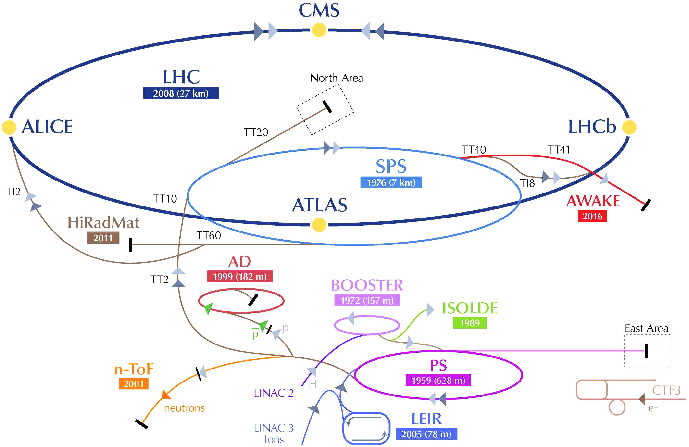
\includegraphics[width=0.75\textwidth]{figures/chapter_ATLAS/LHCAcceleratorComplex}
        \caption{
			This figure shows the accelerator complex of CERN, featuring the experiments and injection chain of the LHC~\cite{Marcastel:1621583}.
        }
        \label{fig:CERNAcceleratorComplex}
    \end{center}
\end{figure}

\subsection{Luminosity}
The instantaneous luminosity is a measure of the rate of events that can be produced under certain detector conditions. It is directly related to the event rate of different processes under production.   
The quantity is given as the following:

\begin{equation}
    L = \frac{F \cdot N^{2}_{p} n_{b} f_{\lambda}}{4\pi\epsilon \beta^{*}}
\end{equation}


\begin{equation}
    \rightarrow = \frac{N_{\textrm{proton in beam 1}} \cdot N_{\textrm{proton in beam 2}} \cdot \textrm{Beam Crossing frequency }}{\textrm{Beam overlap Area}}
\end{equation}

In the formula above, $N_p$ is the number of proton in each beam, $n_{b}$ is the number of bunches per beam, f is the frequency of the beam traveling around the collider, and $\beta^{\*}$ is the beam cross-sectional size at the injection, $\epsilon$ is the beam emittance, F is the beam crossing angle.

The LHC was built to have a peak luminosity at L=$2 \cdot 10^{34}cm^{-2}s^{-1}$, but in most of Run II, it has a nominal value of $10^{34}\texit{cm}^{-2}\textit{s}^{-1}$.

While the instantaneous luminosity is a measure of LHC performance in operation, integrated luminosity, denoted by $\mathcal{L} = \int L dt$ is a measure of the amount of data taken over time.

While an increase in instantaneous luminosity increases the event rate in the experiment, it also increases the pile-up, which is multiple occurrences of interactions that happened simultaneously as the target events. Pile-up cleaning will therefore become an increasingly important task as the LHC instantaneous luminosity increases.

\subsection{Proton Production}
The protons that collide in the LHC came from hydrogen in gaseous form. The electrons are stripped out from getting grated an ion source. Protons formed are grated to make sure they are in the same direction before being sent off to the injection chain for acceleration. 

\subsection{The Injection Chain}
The acceleration of protons after their production is done through the injection chain. It mainly consists of a series of pre-acceleration steps through the different linear booster and booster rings. As the speed and energy of the particle are effectively restricted by both the accelerator ring size as well as magnet strength in a cyclotron accelerator, a dedicated series of smaller rings in ascending order in size are used to accelerate the beam to a higher energy level before the LHC ring.

The protons first go through a linear accelerator named LINAC2 to be accelerated to 50 MeV. After the acceleration, they enter a synchrotron ring called the Proton Synchrotron Booster(SPS). In the SPS, the protons are accelerated to 1.4 GeV at this stage. Subsequently, they are injected into the Proton Synchrotron(PS). The PS accelerates the protons further to 26 GeV and is injected into the Super Proton Synchrotron(SPS), the protons are then further accelerated to 450 GEV and passed onto the LHC ring in \textit{proton bunches}.

These booster rings are existing structures from previous collider experiments~\cite{ATLAS:1999vwa}.

\begin{figure}[!htb]
    \begin{center}
        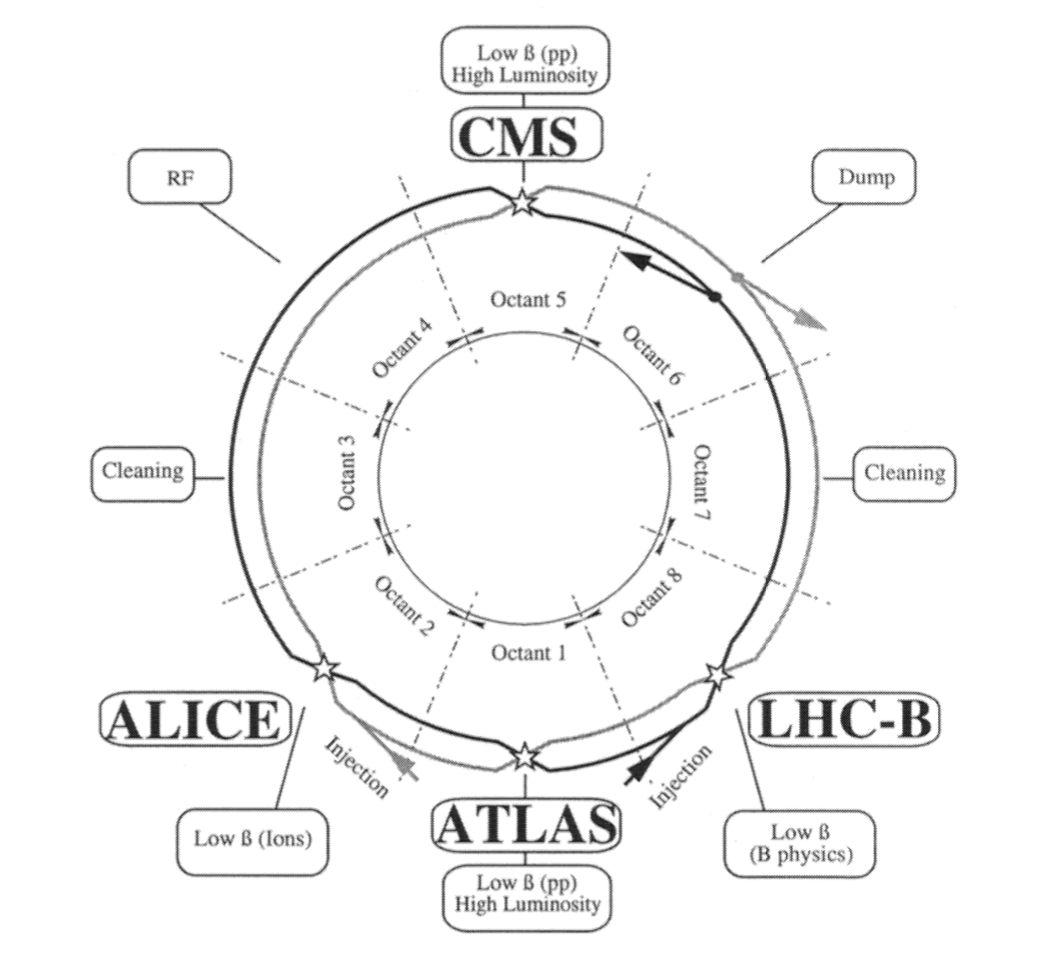
\includegraphics[width=0.75\textwidth]{figures/chapter_ATLAS/LHCRing}
        \caption{
			This figure shows the different parts of the two LHC rings along with its features~\cite{Pettersson:291782}.
        }
        \label{fig:perterson}
    \end{center}
\end{figure}

\subsection{The Radio Frequency Cavities}
After the injection to the LHC, the protons will be further ramped up in energy. Located in IP4 of the LHC main ring, the radio frequency(RF) cavity of the LHC performs the acceleration of particles in the ring. The cavity oscillates its electric field at a fixed 400MHz rate, which accelerates the incoming well-timed protons. In Run II, protons that arrive in the LHC are accelerated from the 450 GeV injection energy to 6.5 TeV in 10 million loops around the LHC, which takes approximately 20 minutes. Other
than accelerating protons, the cavity also modulates the protons' energy: the slowed protons are accelerated and fast one decelerated. They are grouped into proton bunches.

\subsection{The Beam Dump}
The beam dump of the LHC is located in IP6 of the ring. It is designed to abort the beam for when an issue occurred in the LHC to prevent further damage. 

\subsection{The Magnets}
The magnet systems in the LHC provide a way to control the proton beam after its injection from the SPS. The magnets of the LHC serves a couple of different purposes on the LHC: they bend the proton beams for them to stay on the circular cyclotron tunnels; they also focus and align the beam for collision for maximal interaction rate. Due to the high bending power needed, the main ring of the LHC uses NbTi superconducting magnets.  A supporting cryostatics system cools the magnets down to 1.9K
for the superconducting functionalities. The main dipole system is shown to be able to provide a magnetic field of up to 8.4T under this condition. There are a couple of different kinds of magnets along the
LHC, each providing a different function in maintaining the beam for particle collision. The field quality can be summarized by the harmonic multipole analysis: 

\begin{equation}
 B_\textrm{total} = B_y+ iB_x  = B_1\sum_n(b_{n} + i a_{n})(Z/R_{r})^{n-1}
\end{equation}

where $B_y$ is the dipole field in the y-direction, $b_{n}$ and $a_n$ is the multipole coefficients, Z is a complex paramter that describes the coordinates of the magnet, $R_{r}$ is the reference radius, the index of n, refers the to the poles of the magnet field, where n=1 refers to the dipole file, n=2 refers to the quadrupole field and so on. 

\subsubsection*{The Main dipole magnets}
The main magnet is a dipole magnet that bend the proton beams to make them stay on track in the circular tunnels. It can also be used to control the separation of the beam as it focuses and refocuses.
The LHC has two beam pipes for each proton beam going in the opposite direction from the other. The Magnet has a twin-aperture system that allows it to bend both proton beams together. Figure~\ref{fig:dipole} shows the cross-section of the dipole magnet. 

\begin{figure}[!htb]
    \begin{center}
        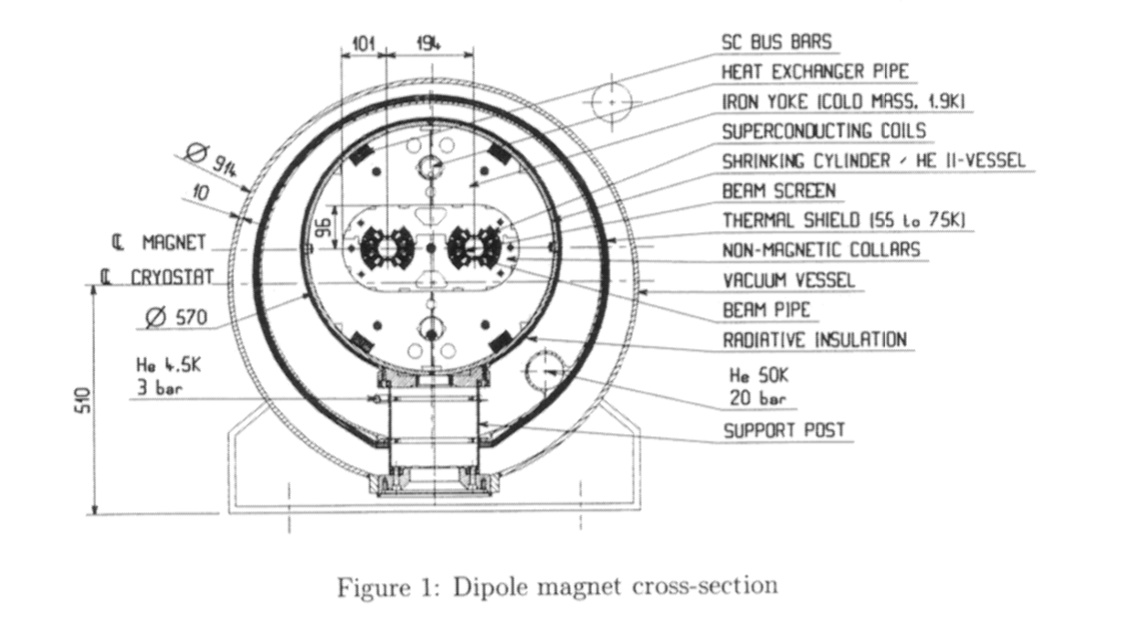
\includegraphics[width=0.75\textwidth]{figures/chapter_ATLAS/DipoleMagnets}
        \caption{
        The cross-section of the dipole magnet~\cite{Bruning:782076}.
        }
        \label{fig:dipole}
    \end{center}
\end{figure}

\subsubsection*{The Quadrupole Magnet}
The Quadrupole magnets are used in the LHC to focuses and defocuses the proton beams for collision. They are built in a way that is much like the main dipole, where single quadrupole magnet is capable of bending two proton beams. Figure~\ref{fig:quadrupole} shows a cross-section of the quadrupole magnet. 

\begin{figure}[!htb]
    \begin{center}
        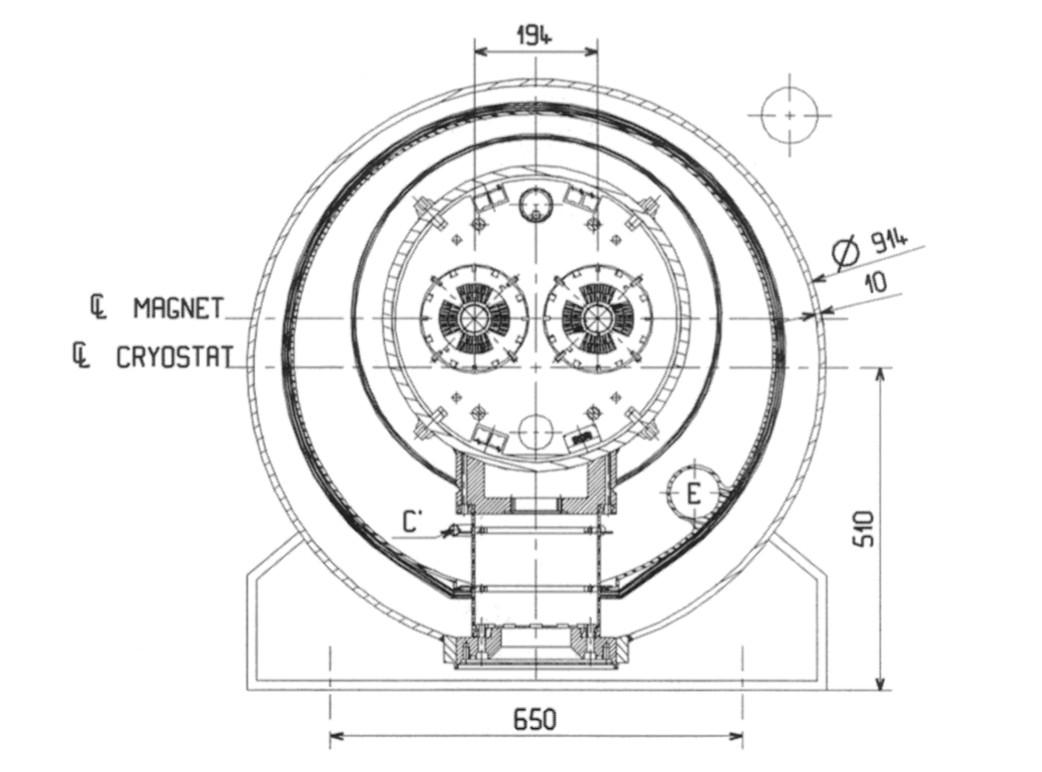
\includegraphics[width=0.75\textwidth]{figures/chapter_ATLAS/QuadrupoleMagnets}
        \caption{
            The cross-section of the quadrupole magnet~\cite{Bruning:782076}.
        }
        \label{fig:quadrupole}
    \end{center}
\end{figure}

\subsubsection*{The Sextupole and Dipole Corrector Magnet}
In addition, there are corrector magnets that correct for the field error of the main magnets mentioned above. More design details can be found in the conceptual design report of the LHC~\cite{Bruning:782076}.

\section{The ATLAS Detector}
\label{ATLAS}
The ATLAS detector is a general-purpose detector. It is the summation of a series of detector systems each produces different tracks to a particle. The ATLAS detector has a special emphasis on the muon system, as the dimuon final state was a main channel for the Higgs discovery. In the following sections, different parts of the detector will be discussed in detail. 

\begin{figure}[!htb]
    \begin{center}
        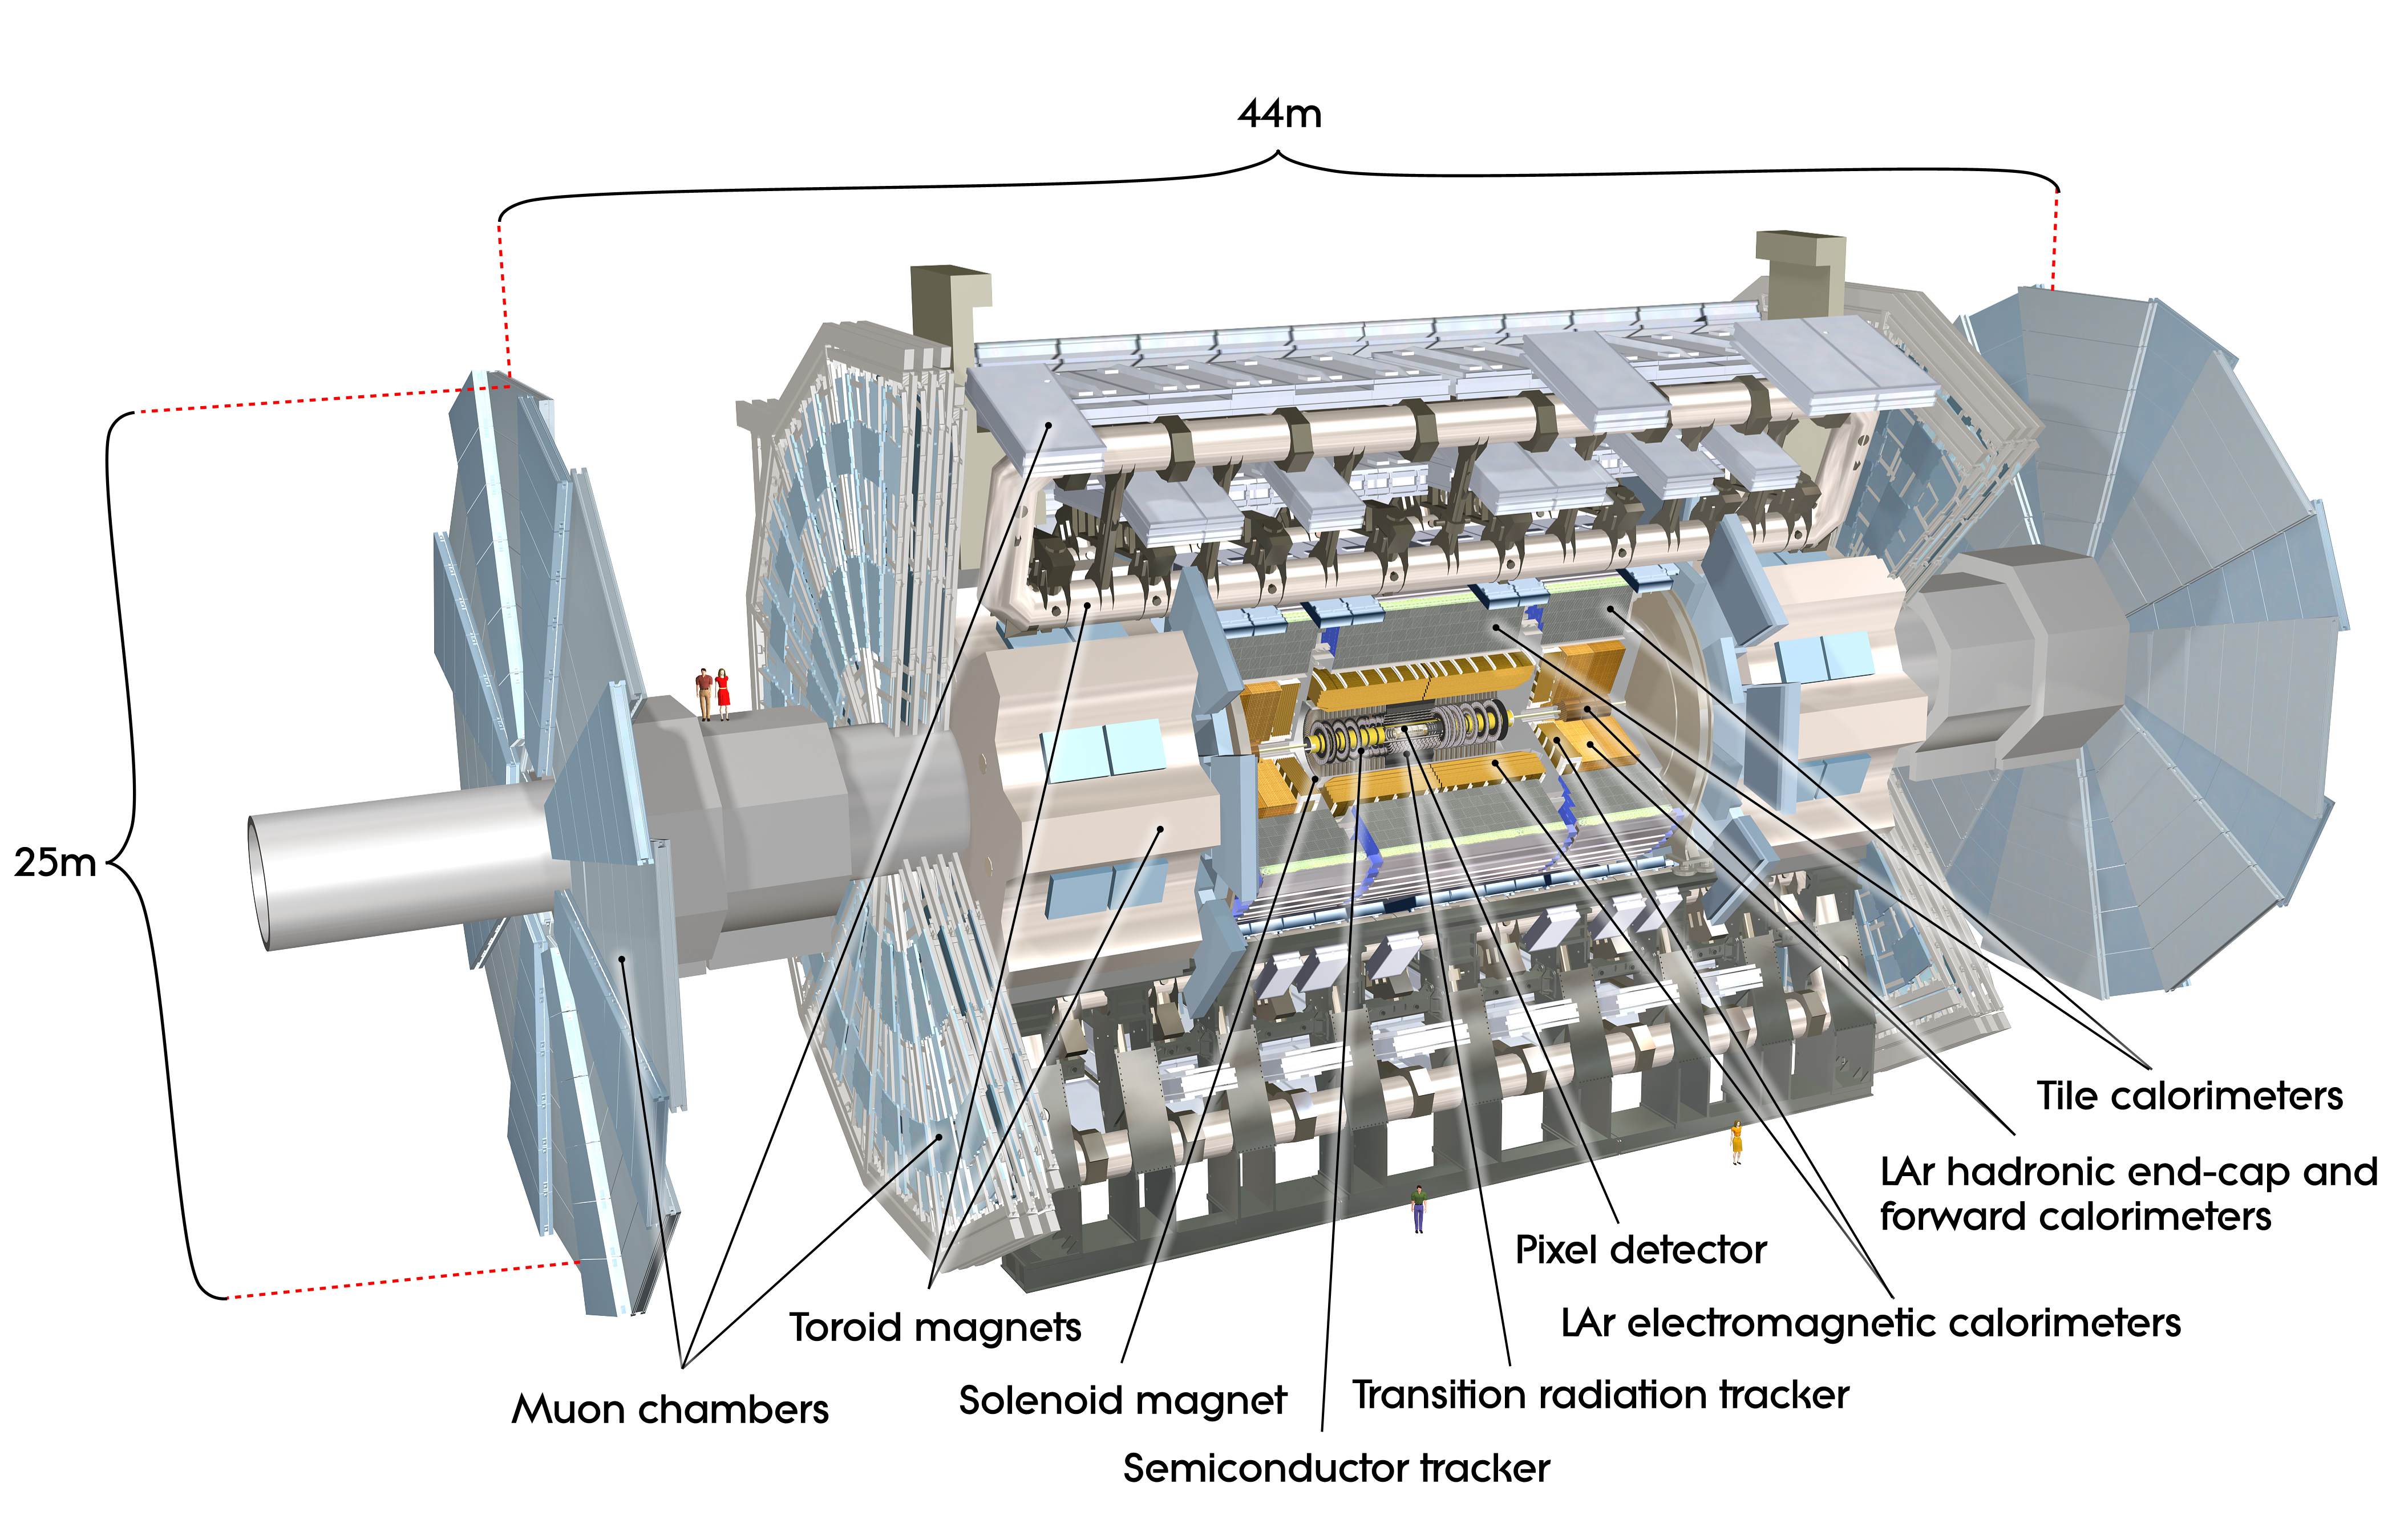
\includegraphics[width=0.75\textwidth]{figures/chapter_ATLAS/ATLASDetector}
        \caption{
			Computer generated image of the ATLAS detector\cite{Pequenao:1095924}. Showing the different parts of the components involved. 
        }
        \label{fig:ATLASDectector}
    \end{center}
\end{figure}


\subsection*{The ATLAS coordinate system}

The ATLAS detector uses a cylindrical coordinate system: Z-$\phi$-$\eta$ to describe the particles location after interactions.
The z-axis runs along the beamline and starts at the origin (center and middle) of the detector. The x-y plane perpendicular to the z-axis described as the transverse plane is represented in the polar coordinate~\ref{fig:Coordinates}. The plane is described by two angles: $\phi$ is the 2$\pi$ azimuthal angle on the x-y plane and the 1$\pi$ polar $\theta$ angle with respect to the z axis is given in term of psuedorapidity, the term is Lorentz invariant and is its conversion to theta is given
by Eq.~\ref{eq:Eta}. The $\delta R$ quantity is used to describe the angular distance between particles, it is defined in Eq.~\ref{eq:deltaR} This quantity is approximately Lorentz invariant. Figure~\ref{fig:Coordinates} shows the ATLAS coordinate system. Figure~\ref{fig:pseudorapidity} shows the pseudorapidity($\eta$) to angle conversion. 

\begin{equation}
    \eta=\ln(\tan(\theta/2))
    \label{eq:Eta}
\end{equation}

\begin{equation}
\delta R=\sqrt{\delta\eta^{2}+\delta\phi^{2}} 
\label{eq:deltaR}
\end{equation}

\begin{figure}[!htb]
    \begin{center}
        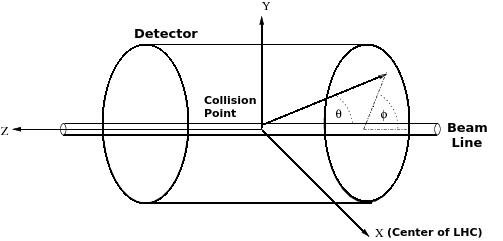
\includegraphics[width=0.75\textwidth]{figures/chapter_ATLAS/Coordinates}
        \caption{
            This figure displays the coordinate of the ATLAS detector system~\cite{2008}.
        }
        \label{fig:Coordinates}
    \end{center}
\end{figure}

\begin{figure}[!htb]
    \begin{center}
        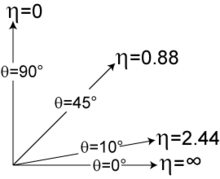
\includegraphics[width=0.45\textwidth]{figures/chapter_ATLAS/pseudorapidity}
        \caption{
            Pseudo-rapidity $\eta$ to angle in degree conversion~\cite{enwiki:1052183914}.
        }
        \label{fig:pseudorapidity}
    \end{center}
\end{figure}



\subsection{Inner Detector}
The inner detector(ID) is the innermost part of the ATLAS detector. Its main function is to record charged particle trajectories. The tracks provide valuable information for the reconstruction of the primary vertices of particle interactions. All four parts of the ID are enclosed by a superconducting solenoid magnet of 2T aligned along the beamline, charged particles are curved into helical trajectories along the beamline. This is used for charge, mass and momentum calculation as well as particle
identification. 

% TODO insert charge to mass trajectory calculation


The inner detector is made up of four different parts. From inside out, the Insertable B Layer, the Pixel detector, the Semi-Conductor Tracker(SCT) and the Transition Radiation Tracker(TRT). 
Its resolution is the highest in the innermost part of the detector and decreases outward. The following is a detailed description of the four parts of their coverage and detector mechanism. 

Closest to the core of the detector is a very high-resolution insertable B layer(IBL). It was inserted after Run I to further extend the pixel detector coverage to $|\eta|< 2.9$. This helps with b-hadron identification through better vertex reconstruction.

Around the IBL is the Pixel detector. It is made of three layers of fine silicon pixels of spatial resolution of 10$\mu$ m in the r-$\phi$ direction and 115$\mu$ m in the z-direction. It provides a cylindrical coverage that covers up to $|\eta|<2.5$. Electron-hole pairs are generated when charged particle passes through the silicon pixel which the signal is then read out through the applied electric field.
Surrounding the pixel detector, there is a silicon microstrip detector called the Semi-Conductor Tracker (SCT), located in radii between 30-51 cm, which is made up of 4 layers of strip silicon sensor. Each SCT layer is made up of two overlapping sets of silicon strips at an angle with one another. The working mechanism of the detector is similar to that of the pixel detector, but the resolution is slightly reduced to 17 $\mu$m in the r-$\phi$ plane and 580 $\mu$ m along the z-axis. 
The outermost part of the ID is called the Transition Radiation Tracker(TRT), made up of gas-filled straws. There are 70 layers in the barrel and 140 layers in each end cap covering up to $|\eta|<2.0$. Each straw tube contains gas that can be ionized by charged particles, the electron formed in the process will then move toward the charged center of the straw to be read out for momentum, trajectory and charge calculation. The TRT also helps with particle identification, as charged particles alsoemit a photon and this probability is related to the Lorentz factor. Lower mass electrons emit more photons than charged hadrons. Therefore, this can be used to identify electrons over hadrons on top of track reconstruction. The TRT has a resolution of 130$\mu$ m in the r-$\phi$ plane.

\begin{figure}[!htb]
    \begin{center}
        \includegraphics[width=0.4\textwidth]{figures/chapter_ATLAS/InnerDetector1}
        \caption{
            This image shows the computer generated image of the inner detector~\cite{Pequenao:1095926}.
        }
        \label{fig:InnerDetector}
    \end{center}
\end{figure}

\begin{figure}[!htb]
    \begin{center}
        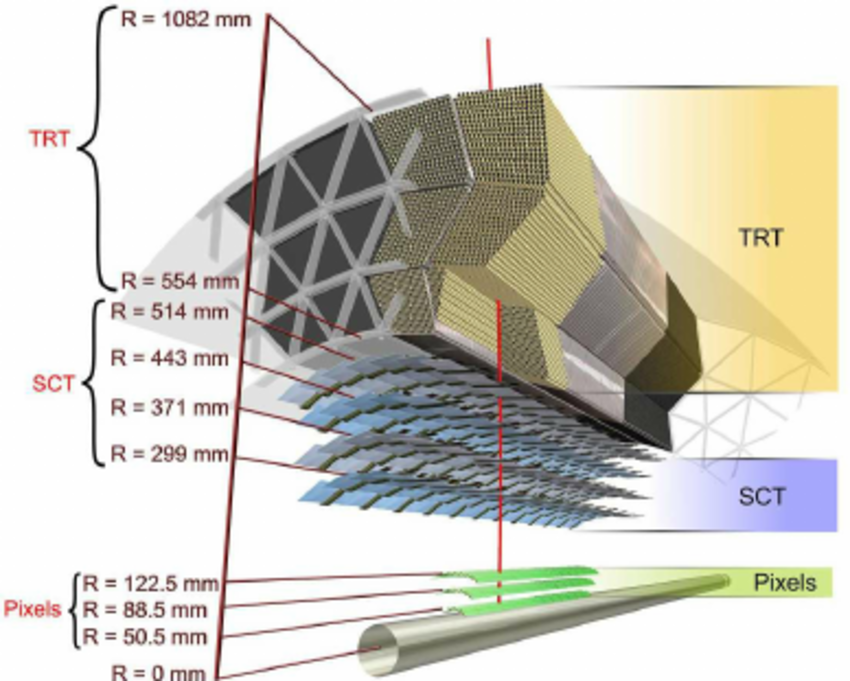
\includegraphics[width=0.75\textwidth]{figures/chapter_ATLAS/InnerDetector2}
        \caption{
            This image shows the computer generated image of the inner detector and its inner layout~\cite{Pequenao:1095926}.
        }
        \label{fig:InnerDetector2}
    \end{center}
\end{figure}

\subsection{Calorimeter}
The main function of the calorimeter is to provide energy measurement for particles. The ATLAS Calorimeter is split into two parts, sorted by the particle interaction method, The Electromagnetic-Calorimeter(ECal) utilizes the electromagnetic interaction and measures energy deposit in the form of electron and photon showers. The Hadronic Calorimeter uses strong hadronic interactions, energy is measured in the form of a hadronic shower in quarks and gluons. Both systems utilize a dense passive material for the particle showering and are sampled through a layer of sensitive active element for detection. Below, different components of the ECAL and the HCAL will be described in detail. 

After tracking, the particle will first reach the ECAL. The first layer is the liquid-argon(LAr) electromagnetic(EM) calorimeter. The passive medium for showering is lead. The endcap portion covers $1.375< |\eta| < 3.2$, and the barrel cover up to $|\eta|<1.475$. The innermost layer has the greatest granularity of 0.003, the second layer has a resolution of 0.025 and the third layer is the most coarse. 

The hadronic calorimeter(HCAL) measures hadron showering in the form of quarks and gluons. The barrel portion of it is made of a tile calorimeter. It uses steel as the passive element for showering and scintillating tiles as the readout active element. 

The forward calorimeter end cap uses LAr for both the ECAL and HCAL, but copper-tungsten is used as the passive layer instead. 


\begin{figure}[!htb]
    \begin{center}
        \includegraphics[width=0.75\textwidth]{figures/chapter_ATLAS/Calorimeter}
        \caption{
            This image shows the computer generated image of the calorimeter and its inner layout~\cite{Pequenao:1095927}.
        }
        \label{fig:Calorimeter}
    \end{center}
\end{figure}

\subsection{Muon Spectrometers}
The muon spectrometer(MS) measures both the trajectory of muons and perform their triggering. The only type of particles that make it past the calorimeters and reach the muon spectrometer are either non-interacting particles, or they are the minimum ionizing particles, muons. Tracking and measurement of muons distinguish the particle from non-interacting particle like neutrinos or Beyond-the-Standard-Model physics candidates like dark matter. 
The muon spectrometer system of ATLAS is surrounded by the superconducting toroid magnets, the barrel toroid provide up to 0.5 T between $1.6 < |\eta|<2.7$ , the end cap toroids provide up to 1T. The magnet bends the particles along the beamline into the end caps.
For precision tracking, the muon system is made up of the Monitored Drift Tubes(MDTs) in both the barrel and the endcap region, in the forward region there is a Cathode Strip Chamber(CSCs) in region $|\eta|>2.7$
For triggering, it uses the Resistive Plate Chamber(RPC) in the barrel and the Thin Gap Chambers (TGCs) in the end cap for fast readout. 

%Comparison with CMS

\begin{figure}[!htb]
    \begin{center}
        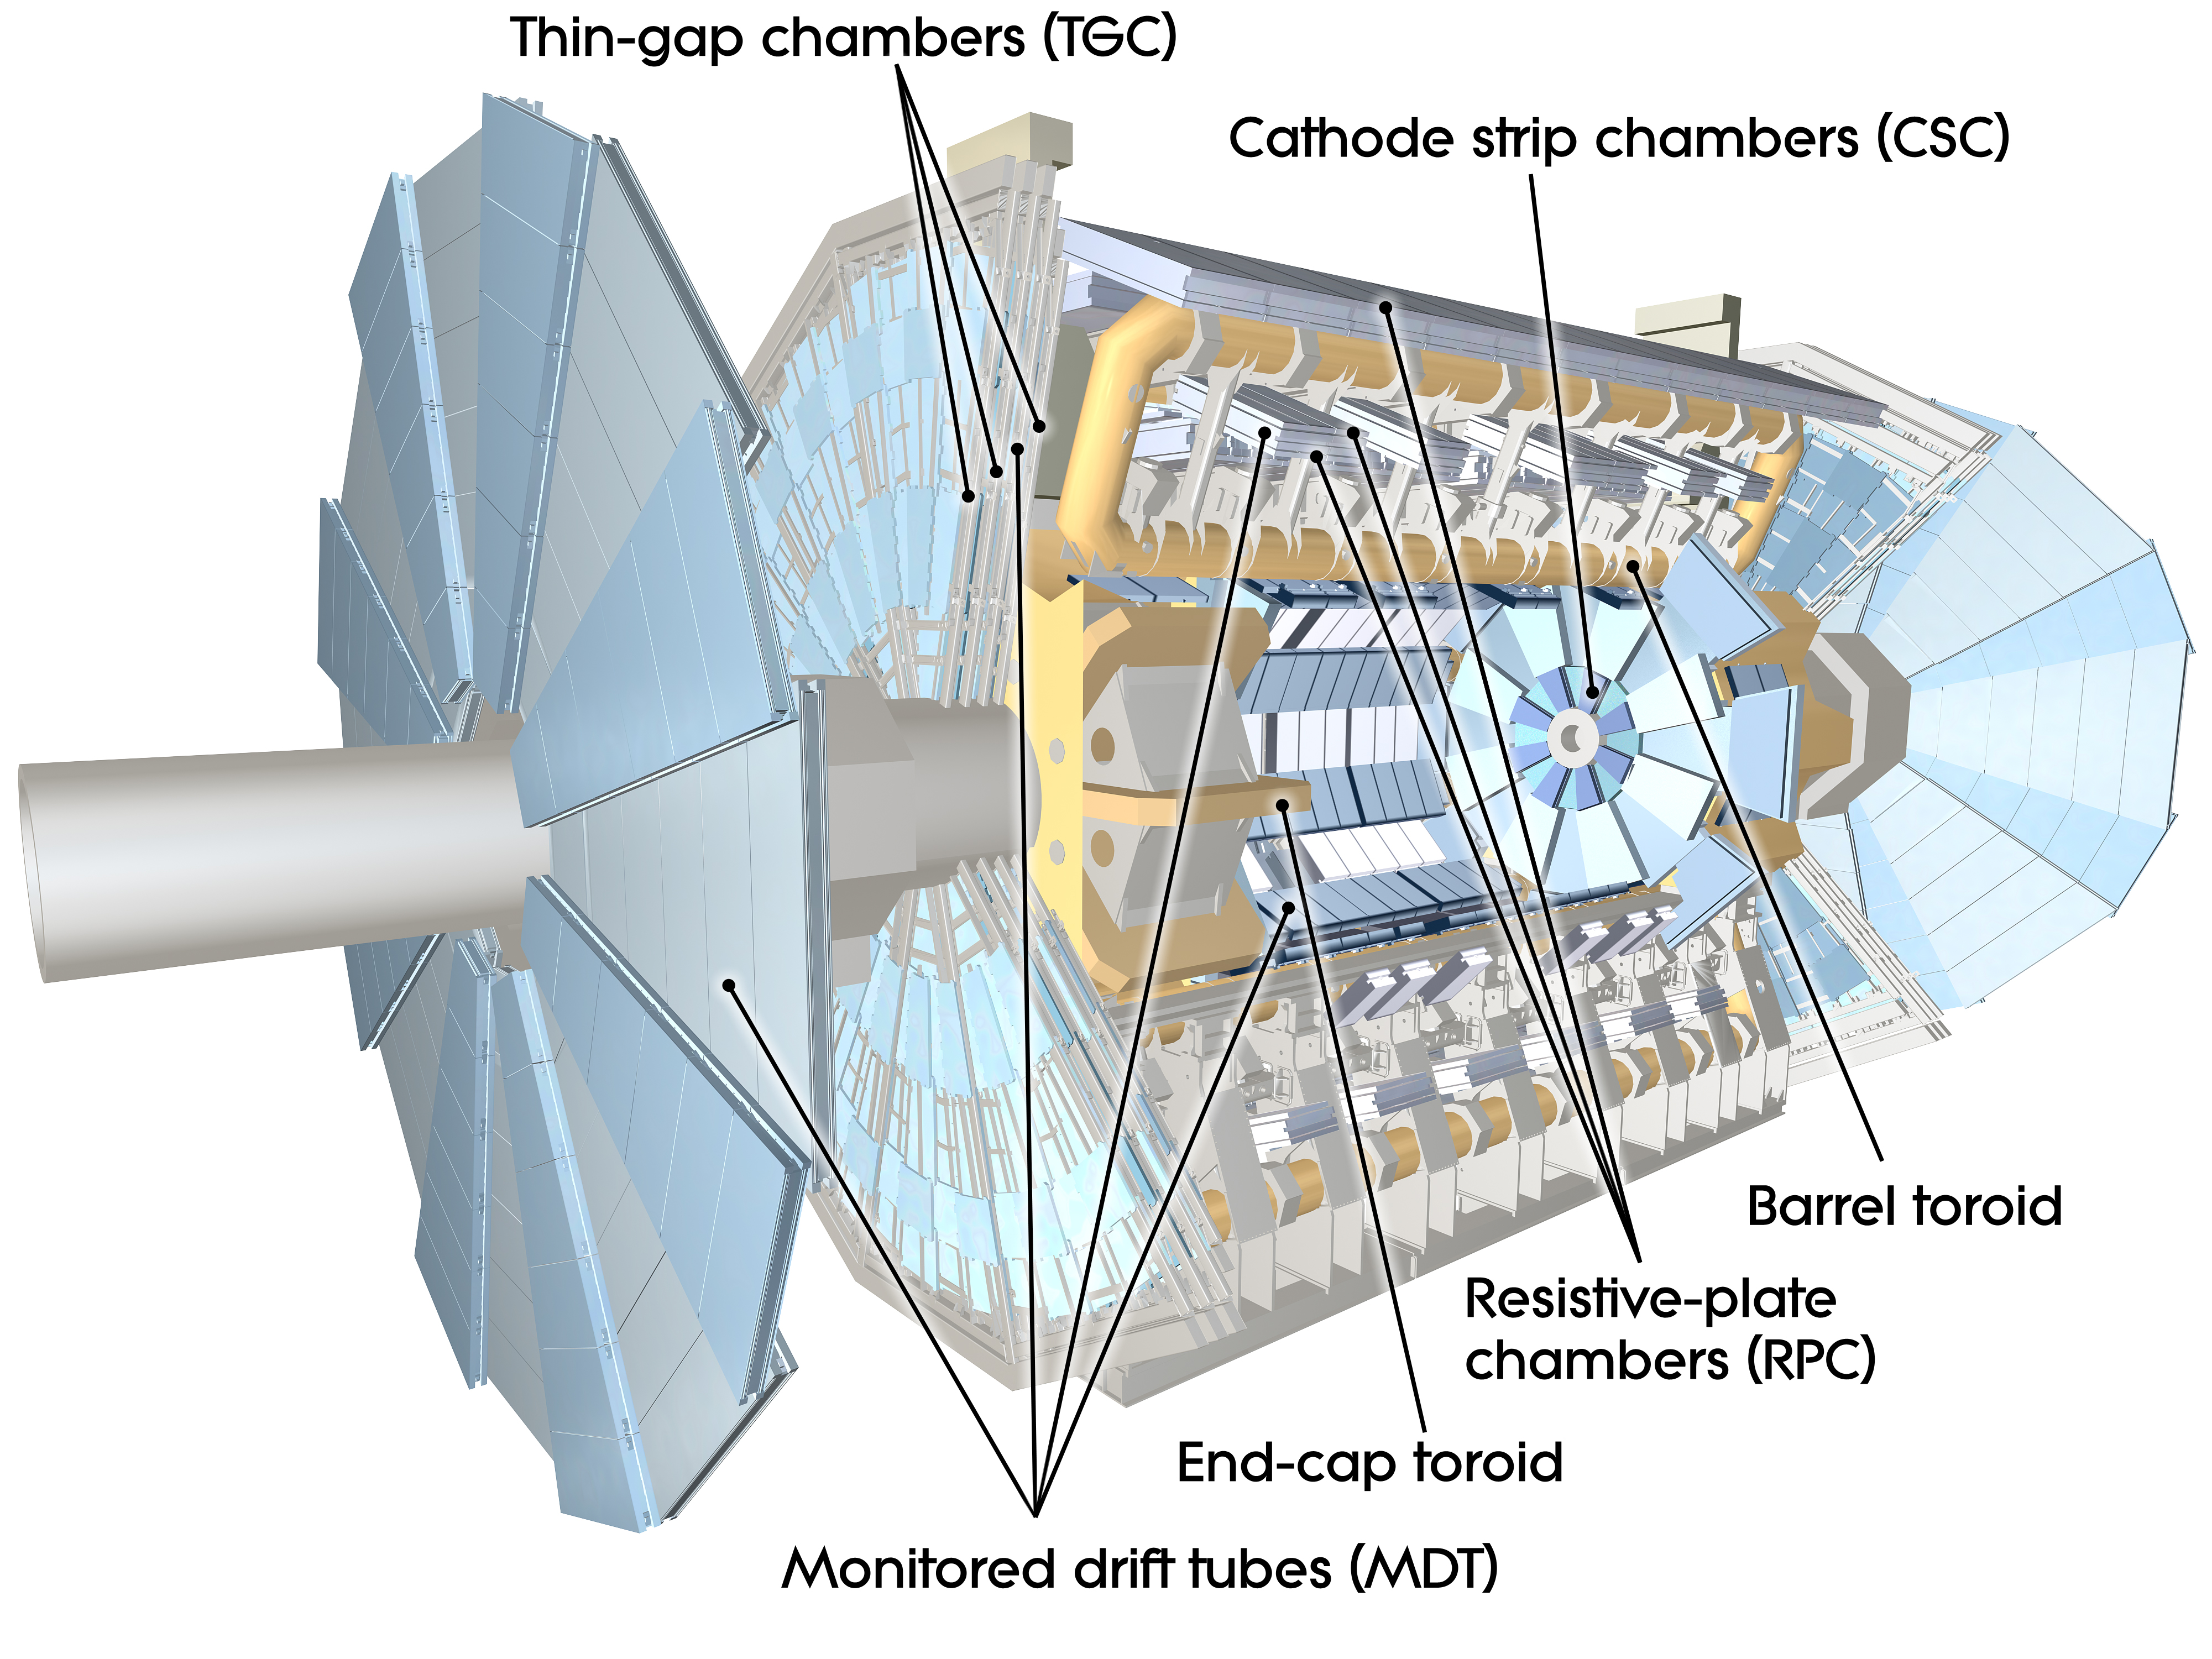
\includegraphics[width=0.75\textwidth]{figures/chapter_ATLAS/MuonSpectrometer}
        \caption{
            This image shows a computer generated image of the muon spectrometer~\cite{Pequenao:1095929}.
        }
        \label{fig:MuonSpectrometer}
    \end{center}
\end{figure}

\section{Data Acquisition of ATLAS}
\label{trigger}
%Data acquisition of ATLAS 
During Run II, the LHC performed proton-proton collision at $\sqrt{s}=13$ TeV at the instantaneous luminosity of $10^{34}cm^{-2}s^{-1}$. An approximate of 33.7 pp interaction per bunch crossing was delivered. 
At this collision rate, not all data could be processed and saved. The process of selecting experimentally interesting events is called ``triggering". In Run II, triggering is administered and controlled by a central trigger processor which assigns different information from detectors to different part of the trigger computing system. There are two levels of triggering in ATLAS Run II, the low level hardware-based trigger is called L1 triggers, the second level software based high level triggering is called the High-level trigger(HLT). 
The L1 trigger filters through the input at 40 MHz to 100kHz. This is done by looking at energy deposits at the calorimeters that could be
candidate leptons, jets, or photons. Muons are triggered by the hits that formed towers in the MS system. 
Events that pass through the L1 trigger will then be passed onto the HLT. The HLT further filters the 100kHz events received to 1kHz for writing to disk for offline analysis. The HLT is software-based. It further defines region-of-interest in detector and filter events that do not fit the trigger selection criteria. High-level objects are created from
the online information and an event loop is used to discard events that do not fulfill the trigger criteria.
Events are saved to ``trigger chains" for later analyses, they are sorted into different analysis derivations with basic criteria applied for different types of analyses. 

\begin{figure}[!htb]
    \begin{center}
        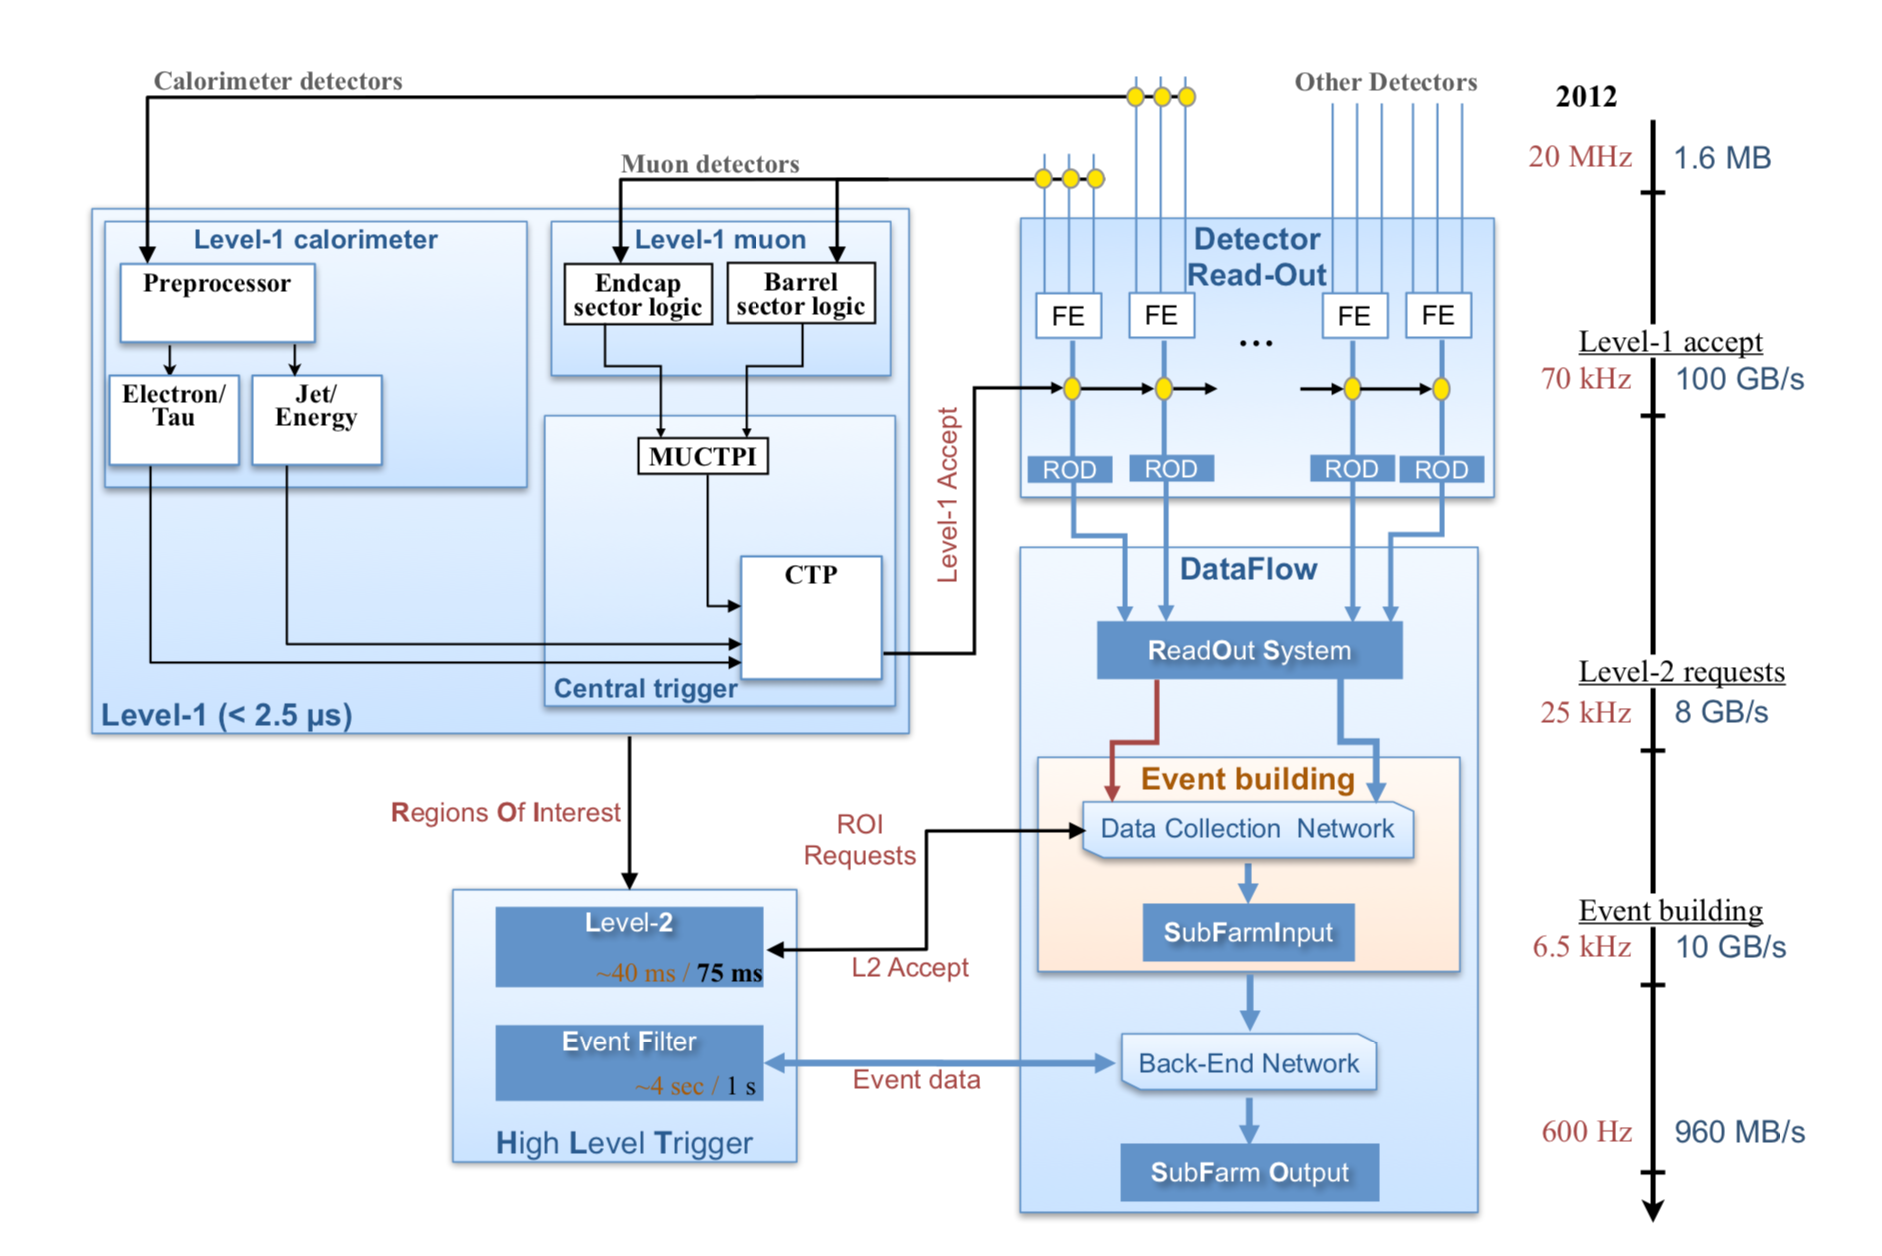
\includegraphics[width=0.75\textwidth]{figures/chapter_ATLAS/TDAQ}
        \caption{
            This image shows the schematic overview of the ATLAS triggering system~\cite{Pequenao:1095929}.
        }
        \label{fig:TDAQ}
    \end{center}
\end{figure}

